\documentclass[10pt,twocolumn]{scrartcl}

\usepackage[utf8]{inputenc}
\usepackage[T1]{fontenc}
\usepackage[ngerman]{babel}

\usepackage{helvet}
\renewcommand{\familydefault}{\sfdefault}

\usepackage{amsmath}
\usepackage{amssymb}

\usepackage{graphicx}
\usepackage{tabularx}

\setlength{\parindent}{0cm}
\setlength{\parskip}{3mm}
\setlength{\textheight}{23.8cm}
\setlength{\headheight}{1cm}
\setlength{\topmargin}{-10mm}

\setlength{\oddsidemargin}{0cm}
\setlength{\evensidemargin}{0cm}
\setlength{\textwidth}{16cm}
\setlength{\columnsep}{8mm}

\usepackage{multicol}
%\usepackage{colortbl}
\usepackage{xcolor}
\definecolor{grau}{gray}{0.95}
\definecolor{dunkelgrau}{gray}{0.85}

%\usepackage[normal]{caption}
%\usepackage{lipsum}

\setlength{\parindent}{5mm}
\setlength{\parskip}{0mm}

\usepackage{float}
\restylefloat{figure}

\renewcommand{\topfraction}{0.75}
\renewcommand{\textfraction}{0.2}

\newcommand{\abs}[1]{\ensuremath{\left\vert#1\right\vert}}

\def\labelitemi{--}
\def\labelitemii{$\bullet$}

%###########################################################
% die Sachen mit der Kopfzeile
\usepackage{lastpage}
\usepackage{fancyhdr}
\fancyhf{} % leere alle Felder
\fancyhead[L]{\footnotesize Simulation des Keplerproblems} % Titel des Aufsatzes
\fancyhead[R]{\footnotesize Constantin Schneider, Nils Wende}
\fancyfoot[C]{\footnotesize \thepage/\pageref{LastPage}}
% \fancyfoot[C]{\footnotesize \thepage}
\renewcommand{\headrulewidth}{0.4pt} % obere Trennlinie
\pagestyle{fancy}
%###########################################################

\newcommand{\ownsection}[1]{\begin{center}\LARGE\bf#1\end{center}}

\begin{document}

\twocolumn[
\ownsection{Simulation des Keplerproblems}

\begin{center}
Constantin Schneider (constantinschneider94@gmail.com), Nils Wende (nils.wende@hotmail.com) \\
Mannheim, November 2015
\end{center}
\vspace*{5mm}
]

% \begin{multicols}{2}
\section{Abstract}
Dieses Kurzpaper erläutert die Simulation des Keplerproblems, d. h. der gegenseitig beeinflussten Bewegung zweier Massen ohne äußere Krafteinwirkung.

Dazu werden Grundlagen wie das Newton'sche Gravitationsgesetz beschrieben, um Gleichungen für die Beschleunigung der Massen herzuleiten. Mit Hilfe des Positions-Verlet-Algorithmus werden dann Geschwindigkeit und Position der Massen iterativ berechnet.

Die berechneten Daten werden mithilfe des zweiten Kepler'schen Gesetzes auf Plausibilität geprüft.


\section{Einleitung}
Das Keplerproblem ist nach dem Naturwissenschaftler Johannes Kepler benannt, der die nach ihm benannten Gesetze anhand von Beobachtungen Anfang des 17. Jahrhunderts aufstellte und veröffentlichte.

Die Kepler'schen Gesetze spielen in mehreren Bereichen der Physik eine wichtige Rolle.

In der Physik wird das Keplerproblem auch allgemein Zweikörperproblem genannt. Dort bezeichnet es das Problem, die Bewegung zweier Körper ohne äußere Krafteinflüsse zu berechnen, dies ist z. B. auch für zwei Atome denkbar. 

Im astronomischen Kontext bezieht es sich z. B. auf die Wechselwirkung zwischen Planet und Mond, Sonne und Planet oder auch in einem Doppelsternsystem. In diesem Paper wird diese Wechselwirkung von Planeten genauer betrachtet.

Da alle äußeren Einflüsse ignoriert werden, stellt das Keplerproblem eine Idealisierung dar, die durch die großen Abstände im Universum -- und die damit geringen exogenen Kräfte -- trotzdem eine gute Näherung ist.

Die Abweichung wird deutlich, sobald die betrachteten Körper in der Realität keine perfekte Kugelgestalt haben. Damit ist auch die Masse der Körper ungleich verteilt, wie es z. B. bei den Gezeiten der Fall ist, wo sich die Masse der Körper abhängig von ihrer Position zueinander verschiebt.

In der Praxis werden die Kepler'schen Gesetze dazu verwendet, Planeten in anderen Sonnensystemen zu prognostizieren, die aufgrund zu großer Distanz zur Erde nicht erkennbar sind. Bei den wechselwirkenden Sternen kommt es ebenfalls zu Bewegungen um den Massenschwerpunkt beider Körper. Aufgrund des Dopplereffekts führt die zusätzliche Bewegung der Sterne zu einer Rotverschiebung, die durch Teleskope beobachtet werden kann. Somit können Rückschlüsse auf die Planeten gemacht werden. Außerdem werden die Kepler'schen Gesetze dazu benutzt, aus gegebenen Messdaten die Bahn eines Himmelskörpers zu berechnen.


\section{Material und Methoden}

\subsection{Newton'sches Gravitationsgesetz}
Das Newton'sche Gravitationsgesetz ist ein physikalisches Gesetz der klassischen Physik zur Berechnung der Kräfte, die zwei Körper aufeinander ausüben. Die Körper werden als Massenpunkte idealisiert. Jeder Massenpunkt wirkt auf jeden anderen Massenpunkt mit einer anziehenden Gravitationskraft ein.

Diese Gravitationskraft ist entlang der Verbindungslinie beider Massenpunkte $m_1$ und $m_2$ gerichtet (siehe Abbildung \ref{fig:newton}) sowie in ihrer Stärke proportional zum Produkt der beiden Massen und umgekehrt proportional zum Quadrat ihres Abstandes $r$. \cite{Wiki15a}

\begin{figure}[t]
\centering
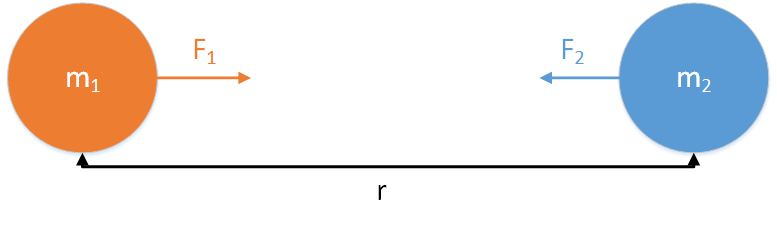
\includegraphics[width=0.45\textwidth]{Bilder/Newton.png}
\caption{Die entgegengesetzten Anziehungskräfte der Massen.}
\label{fig:newton}
\end{figure}

Es gilt also für den Betrag der beiden Kräfte $F_1$ und $F_2$:

\begin{equation}F = \abs{F_1} = \abs{F_2} = G \cdot \frac{m_1 \cdot m_2}{r^2}
\label{eq:newton}
\end{equation}

mit der Gravitationskonstante $G = 6,67408 \cdot 10^{-11} \frac{m^3}{kg \cdot s^2}$.

\subsection{Kepler'sche Gesetze}
Es gibt drei Kepler'sche Gesetze \cite{Max-Planck-Gesellschaft2015} :
\begin{enumerate}
\item  Die Umlaufbahnen zweier Körper haben die Form einer Ellipse, in deren einem gemeinsamen Brennpunkt der Masseschwerpunkt des Systems liegt. 
\item Der Fahrstrahl Objekt -- Baryzentrum (Massenschwerpunkt des Systems) überstreicht in gleichen Zeiten die gleiche Fläche.

Abbildung \ref{fig:kepler2} stellt dies dar. Das Baryzentrum ist hier gleichzeitig auch einer der Brennpunkte der Ellipse. Dies ist näherungsweise der Fall, wenn der Massenunterschied zwischen den betrachteten Objekten sehr groß ist, z. B. bei Erde und Sonne.

\begin{figure}[t]
\centering
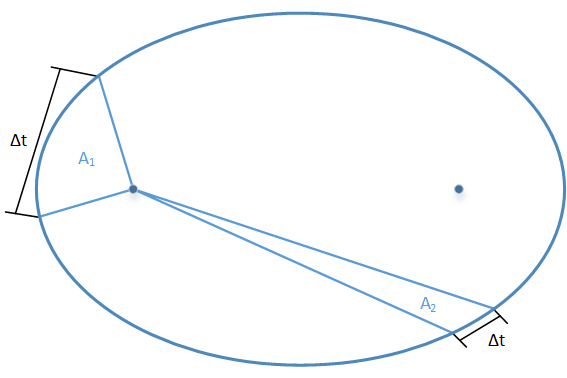
\includegraphics[width=0.45\textwidth]{Bilder/kepler2.png}
\caption{Zweites Kepler'sches Gesetz: $A_1$ und $A_2$ sind bei gleichem $\Delta t$ gleich groß.}
\label{fig:kepler2}
\end{figure}

\item Teilt man das Quadrat der Umlaufzeit $T$ eines Himmelskörpers durch die dritte Potenz seines mittleren Abstandes $a$ zur Sonne, ergibt sich für jeden Planeten im Sonnensystem derselbe Wert $C$

\begin{equation}C = \frac{T^2}{a^3}
\label{eq:kepler3}
\end{equation}

Für die Sonne gilt $C_S = 2,97 \cdot 10^{-19} \frac{s^2}{m^3}$.

\end{enumerate}


\subsection{Herleitung der Beschleunigungsgleichungen}
In einer Ebene bewegen sich zwei Massenpunkte $m_1$ und $m_2$. Da sich beide Massen abhängig von der Zeit $t$ bewegen, werden ihre Positionskoordinaten als $(x_1(t), y_1(t))$ und $(x_2(t), y_2(t))$ beschrieben. Abbildung \ref{fig:abb1} stellt diese Situation zu einem bestimmten Zeitpunkt $t$ dar.

\begin{figure}[t]
\centering
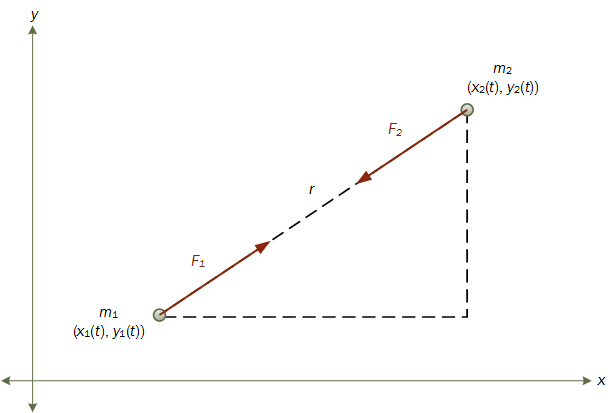
\includegraphics[width=0.45\textwidth]{Bilder/abb1.png}
\caption{$m_1$ und $m_2$ haben den Abstand $r$ zueinander und ziehen sich mit den vom Betrag her gleichen Kräften $F_1$ und $F_2$ an. \cite{MicrosoftOJ}}
\label{fig:abb1}
\end{figure}

Da $F_1$ eine vektorielle Größe ist, kann sie auch, wie in Abbildung \ref{fig:abb2} zu sehen, komponentenweise als $F_x$ und $F_y$ ausgedrückt werden.

\begin{figure}[t]
\centering
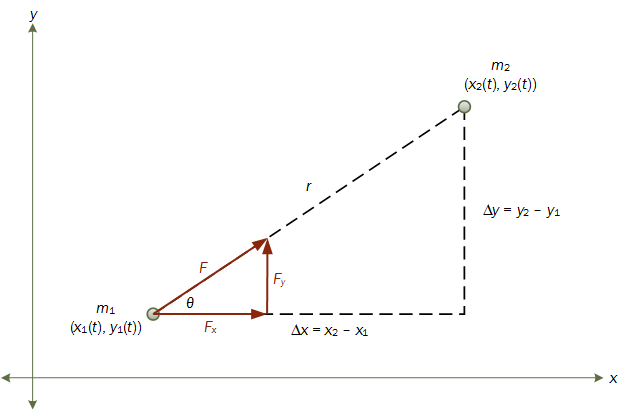
\includegraphics[width=0.45\textwidth]{Bilder/abb2.png}
\caption{Die Komponenten von $F_1$, anliegend an $m_1$. \cite{MicrosoftOJ}}
\label{fig:abb2}
\end{figure}

Trigonometrisch ergibt sich:

\begin{equation}F_x = F \cdot \cos \theta
\label{eq:2}
\end{equation}

\begin{equation}F_y = F \cdot \sin \theta
\label{eq:3}
\end{equation}

Das größere Dreieck zeigt, dass

\begin{equation}\cos \theta = \frac{\Delta x}{r} = \frac{x_2 - x_1}{r}
\label{eq:4}
\end{equation}

\begin{equation}\sin \theta = \frac{\Delta y}{r} = \frac{y_2 - y_1}{r}
\label{eq:5}
\end{equation}

Für $F_x$ ergibt sich damit durch Einsetzen der Gleichungen \eqref{eq:newton} und \eqref{eq:4}:

\begin{equation}F_x = G \cdot \frac{m_1 \cdot m_2 \cdot (x_2 - x_1)}{r^3}
\label{eq:8}
\end{equation}

Das zweite Newton'sche Gesetz besagt, dass

\begin{equation}F = m \cdot a
\label{eq:9}
\end{equation}

Betrachtet man nur die x-Komponente der Vektoren $F$ und $a$ in Bezug auf die Masse $m_1$, ergibt sich:

\begin{equation}F_x = m_1 \cdot a_x
\label{eq:10}
\end{equation}

Wir haben nun mit den Gleichungen \eqref{eq:8} und \eqref{eq:10} zwei Ausdrücke für $F_x$:

\begin{equation}
	\begin{aligned}
		F_x {} & = m_1 \cdot a_x \\
  			& = G \cdot \frac{m_1 \cdot m_2 \cdot (x_2 - x_1)}{r^3}
	\end{aligned}
\label{eq:11}
\end{equation}

Dividiert man durch $m_1$, erhält man:

\begin{equation}a_x = G \cdot \frac{m_2 \cdot (x_2 - x_1)}{r^3}
\label{eq:12}
\end{equation}

Der Abstand $r$ zwischen den beiden Massen berechnet sich nach dem Satz des Pythagoras durch:

\begin{equation}
	\begin{aligned}
		r {} & = \sqrt{(\Delta x)^2 + (\Delta y)^2} \\
  			& = [(x_2-x_1)^2 + (y_2-y_1)^2]^\frac{1}{2}
	\end{aligned}
\label{eq:13}
\end{equation}

Einsetzen in Gleichung \eqref{eq:12} ergibt:

\begin{equation}a_x = G \cdot \frac{m_2 \cdot (x_2 - x_1)}
									{[(x_2-x_1)^2 + (y_2-y_1)^2]^\frac{3}{2}}
\label{eq:14}
\end{equation}

Mit dieser Gleichung kann die Beschleunigung von $m_1$ in x-Richtung in Abhängigkeit der Koordinaten der Massen berechnet werden \cite{MicrosoftOJ}.

Analog lässt sich die Gleichung für die y-Komponente der Beschleunigung von $m_1$ aufstellen:

\begin{equation}a_y = G \cdot \frac{m_2 \cdot (y_2 - y_1)}
									{[(x_2-x_1)^2 + (y_2-y_1)^2]^\frac{3}{2}}
\label{eq:15}
\end{equation}

Für $m_2$ sind die Beschleunigungsgleichungen ähnlich:

\begin{equation}a_x = G \cdot \frac{m_1 \cdot (x_1 - x_2)}
								{[(x_2-x_1)^2 + (y_2-y_1)^2]^\frac{3}{2}}
\label{eq:16}
\end{equation}

\begin{equation}a_y = G \cdot \frac{m_1 \cdot (y_1 - y_2)}
									{[(x_2-x_1)^2 + (y_2-y_1)^2]^\frac{3}{2}}
\label{eq:17}
\end{equation}

Zur Vereinfachung schreiben wir die vorangegangenen Gleichungen so, wobei die tiefgestellte Ziffer jeweils für die Masse $m_1$ oder $m_2$ steht:

\begin{equation}a_{1_x} := G \cdot \frac{m_2 \cdot (x_2 - x_1)}
			{\alpha}
\label{eq:18}
\end{equation}

\begin{equation}a_{1_y} := G \cdot \frac{m_2 \cdot (y_2 - y_1)}
			{\alpha}
\label{eq:19}
\end{equation}

\begin{equation}a_{2_x} := G \cdot \frac{m_1 \cdot (x_1 - x_2)}
			{\alpha}
\label{eq:20}
\end{equation}

\begin{equation}a_{2_y} := G \cdot \frac{m_1 \cdot (y_1 - y_2)}
			{\alpha}
\label{eq:21}
\end{equation}

mit $\alpha := [(x_2-x_1)^2 + (y_2-y_1)^2]^\frac{3}{2}$ und $\alpha \neq 0$.\\

Diese Gleichungen stellen die Beschleunigung eines Körpers in Abhängigkeit seiner Position dar \cite{MicrosoftOJ}.

Um Geschwindigkeit und Position zu einem späteren Zeitpunkt zu bestimmen, nutzen wir den Positions-Verlet-Algorithmus, der nachfolgend näher erklärt wird.


\subsection{Positions-Verlet-Algorithmus}
Der Positions-Verlet-Algorithmus ist ein sogenannter Leapfrog-Algorithmus, welcher zur numerischen Integration der Newton'schen Bewegungsgleichungen genutzt werden kann.

Abbildung \ref{fig:leapfrog} visualisiert die Idee hinter einem Leapfrog-Algorithmus. Mit den Startwerten $x_0$ und $v_\frac{1}{2}$ werden abwechselnd die Position und Geschwindigkeit der nächsten Iteration bestimmt, die hüpfende Bewegung der Pfeile erinnert dabei an das Bockspringen (engl. {\it leapfrog}).

\begin{figure}[t]
\centering
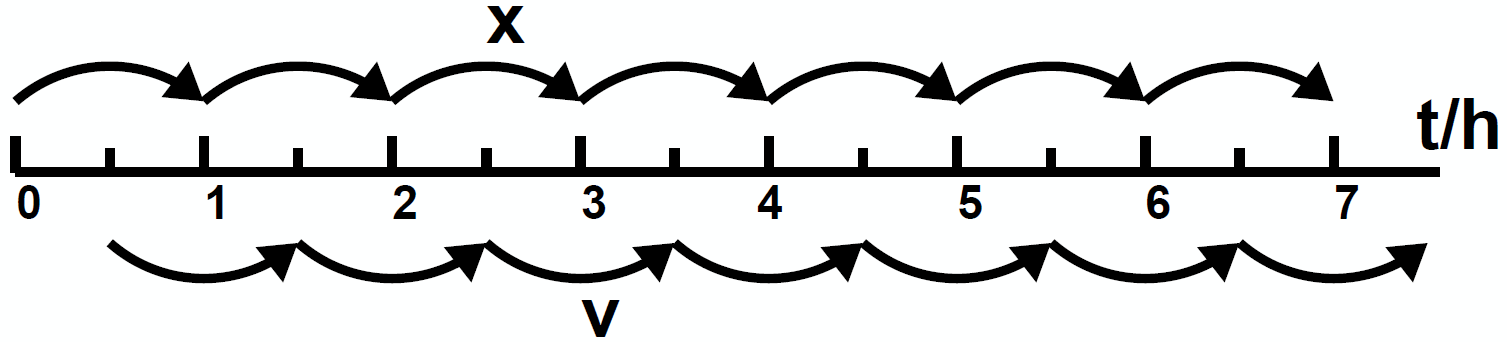
\includegraphics[width=0.45\textwidth]{Bilder/leapfrog.png}
\caption{Die Struktur der Leapfrog-Methode. (\cite{Young14}, S. 2)}
\label{fig:leapfrog}
\end{figure}

Beim Positions-Verlet-Algorithmus wird allerdings entgegengesetzt zu Abbildung \ref{fig:leapfrog} vorgegangen:

Es wird erst ein halber Schritt für $x$, ein ganzer Schritt für $v$ und dann wieder ein halber Schritt für $x$ gemacht.

Dabei kommen folgende Gleichungen zum Einsatz, wobei das hochgestellte $i$ den Index der jeweiligen Masse darstellt (\cite{Young14}, S. 5):

\begin{equation}x_{n+\frac{1}{2}}^i := x_n^i + \frac{1}{2} \cdot \Delta t \cdot v_n^i
\label{eq:22}
\end{equation}

\begin{equation}v_{n+1}^i := v_n^i + \Delta t \cdot a_{n+\frac{1}{2}}^i
\label{eq:23}
\end{equation}

\begin{equation}x_{n+1}^i := x_{n+\frac{1}{2}}^i + \frac{1}{2} \cdot \Delta t \cdot v_{n+1}^i
\label{eq:24}
\end{equation}

Um die Genauigkeit zu verbessern, wird bei der ersten Iteration Gleichung \eqref{eq:22} durch diese Gleichung ersetzt \cite{MicrosoftOJ}:

\begin{equation}x_{\frac{1}{2}}^i := x_0^i + \frac{1}{2} \cdot \Delta t \cdot v_0^i
+ \frac{1}{4} \cdot (\Delta t)^2 \cdot a_0^i
\label{eq:25}
\end{equation}


\subsection{Simulationsalgorithmus}
Die Nutzung des Positions-Verlet-Algorithmus führt zu folgendem Ablauf \cite{MicrosoftOJ}:

\begin{enumerate}
	\item Wähle einen kleinen Zeitschritt $\Delta t$.
	\item Wähle die Masse und komponentenweise die initialen Positions- und Geschwindigkeitswerte der Körper.
	\item Berechne die initialen Beschleunigungswerte $a_0^i$ mit den Gleichungen \eqref{eq:18} bis \eqref{eq:21}.
	\item Berechne mit den Werten der $a_0^i$ mit Gleichung \eqref{eq:25} die Werte von $x_{\frac{1}{2}}^i$.
	\item Wiederholung bis manueller Abbruch (Startwert $n:=0$):
	\begin{enumerate}
		\item Berechne mit den Werten der $x_{n+\frac{1}{2}}^i$ mit den Gleichungen \eqref{eq:18} bis \eqref{eq:21} die Werte der $a_{n+\frac{1}{2}}^i$.
		\item Berechne mit den Werten der $a_{n+\frac{1}{2}}^i$ mit Gleichung \eqref{eq:23} die Werte der $v_{n+1}^i$.
		\item Berechne mit den Werten der $v_{n+1}^i$ mit Gleichung \eqref{eq:24} die Werte der $x_{n+1}^i$.
		\item Zeige die neuen Positionen der Massen an.
		\item Berechne mit den Werten der $x_{n+1}^i$ mit Gleichung \eqref{eq:22} die Werte der $x_{n+\frac{3}{2}}^i$.
		\item Setze $n := n+1$.
	\end{enumerate}
\end{enumerate}



\section{Durchführung}
Nutzen wir den Algorithmus, um beispielsweise das Erde-Mond-System zu simulieren, können wir die folgenden Initialwerte (einige aus \cite{nasa15} entnommen, $v_{y_0}$ der Erde experimentell bestimmt) setzen:

\begin{itemize}
	\item Erde:
	\begin{itemize}
		\item $m := 5,9726 \cdot 10^{24} kg$
		\item $x_0 := 0,4055 \cdot 10^{9} m$
		\item $y_0 := 0,4333 \cdot 10^{9} m$
		\item $v_{x_0} := 0 \frac{m}{s}$
		\item $v_{y_0} := -11,86188 \frac{m}{s}$
	\end{itemize}
	\item Mond:
	\begin{itemize}
		\item $m := 7,3492 \cdot 10^{22} kg$
		\item $x_0 := 0 m$
		\item $y_0 := 0,4333 \cdot 10^{9} m$
		\item $v_{x_0} := 0 \frac{m}{s}$
		\item $v_{y_0} := 964 \frac{m}{s}$
	\end{itemize}
\end{itemize}

Wir wählen $\Delta t := 1h$ und führen zwischen jeder Ausgabe der Werte die Berechnung 6-mal hintereinander durch, woraus sich ein effektives $\Delta t$ von $6h$ ergibt.

\section{Ergebnis}
Das Ergebnis der Simulation wird in Abbildung \ref{fig:sim} dargestellt. Beide Massen bewegen sich jeweils auf einer Ellipsenbahn um das gemeinsame Baryzentrum durch den Raum. Abbildung \ref{fig:zoom} zeigt das Ergebnis vergrößert auf die Bahn der Erde.

Die Simulation entspricht dem zweiten Kepler'schen Gesetz. Für unser $\Delta t = 6 h$ erhält man für die als Dreieck angenäherte Fläche des Fahrstrahls zwischen Erde und Baryzentrum einen Wert zwischen $6,3106 \cdot 10^{11} m^2$ und $6,3114 \cdot 10^{11} m^2$, für die Fläche zwischen Mond und Baryzentrum einen Wert zwischen $4,1679 \cdot 10^{15} m^2$ und $4,1684 \cdot 10^{15} m^2$.

Beide unterscheiden sich jeweils nur um $8 \cdot 10^7 m^2$ bzw. $5 \cdot 10^{11} m^2$ sind damit näherungsweise konstant. Die Abweichungen können mit der Dreiecksnäherung erklärt werden.

\begin{figure*}[t]
\centering
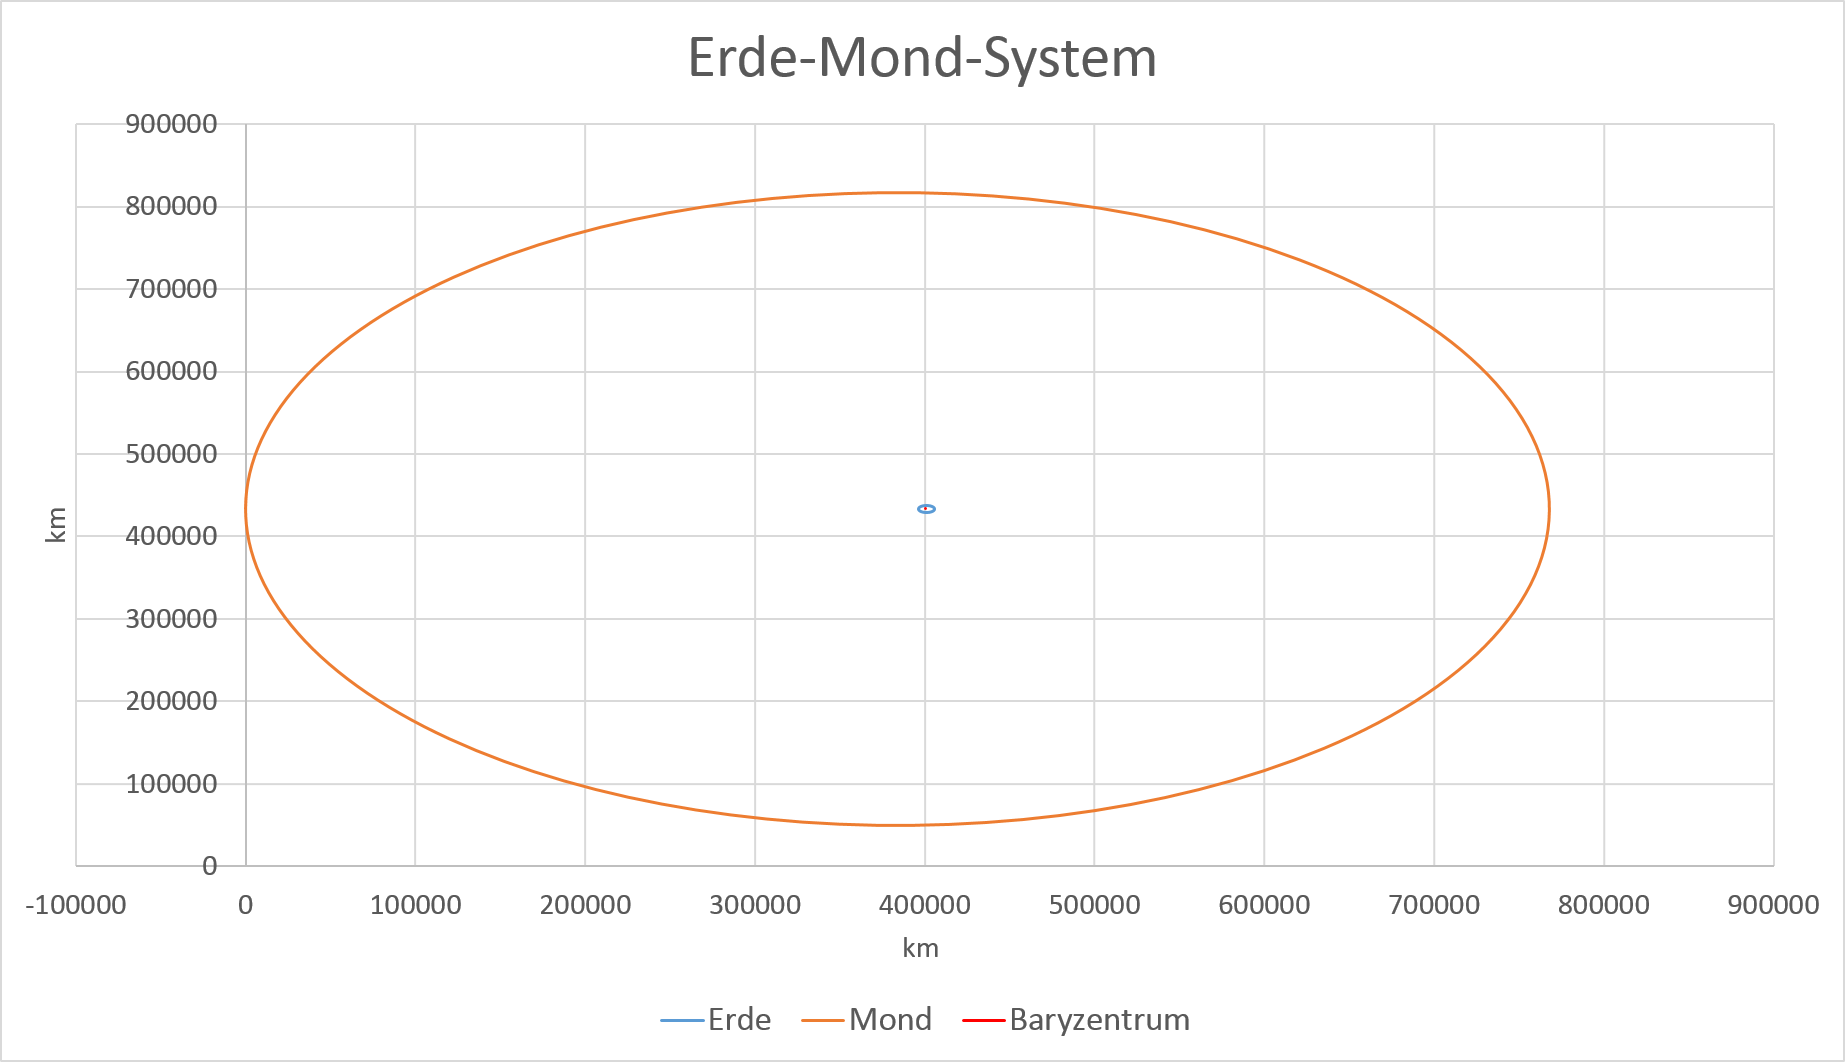
\includegraphics[width=0.90\textwidth]{Bilder/simulation.png}
\caption{Ergebnis der Simulation des Erde-Mond-Systems.}
\label{fig:sim}
\end{figure*}

\begin{figure*}[t]
\centering
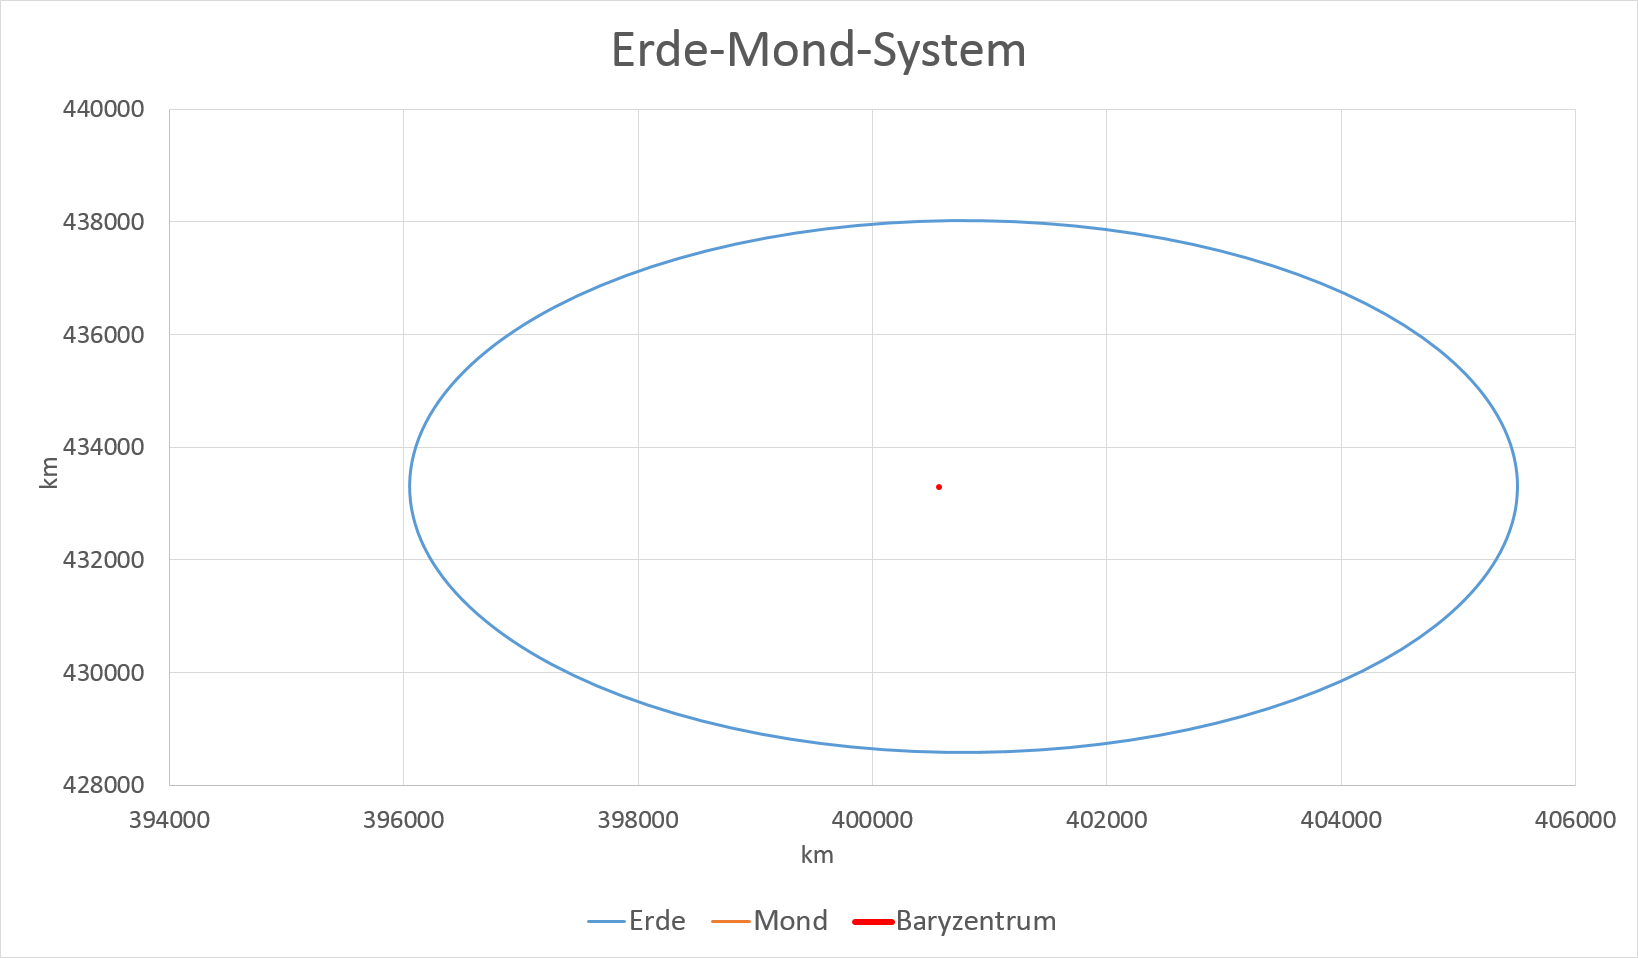
\includegraphics[width=0.90\textwidth]{Bilder/zoomErde.png}
\caption{Zoom auf die Erdbahn mit Baryzentrum.}
\label{fig:zoom}
\end{figure*}

Experimentell ließ sich der Zusammenhang der Körpermassen ($m_1$, $m_2$), sowie der Körpergeschwindigkeiten ($v_1$, $v_2$)

\begin{equation}\frac{m_1}{m_2} = \frac{\abs{v_2}}{\abs{v_1}}
\label{rot}
\end{equation}

erkennen.

Für das hier simulierte Erde-Mond-System liegt dieser Quotient bei $81,26871$.


\section{Diskussion}
Es hätte auch der Verlet-Algorithmus (\cite{Young14}, S. 5f) benutzen werden können, da wir die Geschwindigkeiten der Körper während der Simulation nicht auswerten müssen.

Dieser ist allerdings bei sehr kleinen $\Delta t \ll 1s$ anfälliger für Rundungsfehler und wird daher von uns nicht benutzt.


Die Initialgeschwindigkeit der Erde ist nicht ganz korrekt gewählt. Dies zeigt sich darin, dass die y-Position des Baryzentrums mit $0,0108 \frac{m}{h}$ langsam ansteigt. Je näher die gewählte Geschwindigkeit an die tatsächlich benötigte Geschwindigkeit angenähert wird, desto geringer wird die Bewegung des Baryzentrums.

Zusammenfassend lässt sich sagen, dass der Algorithmus zur Berechnung der Flugbahnen erfolgreich anhand von grundlegenden Gesetzesmäßigkeiten hergeleitet wurde. Die Kepler'schen Gesetze wurden vorgestellt und das Ergebnis ist eine Simulation der Flugbahnen von Sonne und Mond, deren Korrektheit anhand des zweiten Kepler'schen Gesetzes verifiziert wurde. 

Zusätzlich hätten die Ergebnisse auch mit den anderen beiden Kepler'schen Gesetzen überprüft werden können.

Die Simulation kann auch auf das Dreikörperproblem erweitert werden. Es beschreibt die gegenseitige Beeinflussung dreier Körper und wird analog behandelt, die Berechnung wird entsprechend komplexer. Theoretisch könnten sogar beliebig viele Körper betrachtet werden.

Ein weiteres Maß an Komplexität wird erreicht, wenn die Körper nicht als Massenpunkte angesehen werden, sondern als Körper mit einer Ausdehnung im Raum. Diese kann zusätzlich auch unregelmäßig oder veränderbar sein, was zum Beispiel bei Erde und Mond der Fall ist, denn das Wasser auf der Erde wird durch die Wechselwirkung mit dem Mond bewegt (Gezeiten).

Es ist auch eine genauere Betrachtung der Einflüsse der Relativitätstheorie möglich, die bei zunehmender Geschwindigkeit der Körper eine bedeutendere Rolle spielt.




\begin{thebibliography}{99}
\bibitem{nasa15}D. R. Williams: {\itshape Moon Fact Sheet}, Greenbelt 2015, http://nssdc.gsfc.nasa.gov/planetary\\/factsheet/moonfact.html
\bibitem{Young14}P. Young: {\itshape The leapfrog method and other “symplectic” algorithms for integrating Newton’s laws of motion}, o.O. 2014
\bibitem{MicrosoftOJ}MSDN: {\itshape The physics and equations of the two- and three-body problem}, o.O. o.J., https://msdn.microsoft.com/en-gb/library/dn528554(v=vs.85).aspx
\bibitem{Max-Planck-Gesellschaft2015}Max-Planck-Gesellschaft zur Förderung der Wissenschaften e.V.: {\it Kepler'sche Gesetze}, 2015, http://www.einstein-online.info/lexikon/KeplerGesetze
\bibitem{Wiki15a}Wikipedia: {\itshape New\-ton\-sches Gravitationsgesetz}, o.O. 2015, https://de.wikipedia.org\\/w/index.php?title=Newtonsches\\\_Gravitationsgesetz\&oldid=147646332
%\bibitem{Wiki15b}Wikipedia: {\it Keplersche Gesetze, 2. Keplersches Gesetz (Flächensatz)}, o.O. 2015b,\\https://de.wikipedia.org/w/index.php\\?title=Keplersche\_Gesetze\\\&oldid=145952164\#2.\_Keplersches\_Gesetz\\\_.28Fl.C3.A4chensatz.29

\end{thebibliography}

\end{document}
